\documentclass[prd,floatfix,nofootinbib,longbibliography,notitlepage,superscriptaddress]{revtex4-1}

% voodoo for arXiv scripts, following must appear on line 5 or earlier
\pdfoutput=1

% I put amsmath... in usepackage statements instead of documentclass
% because AUCTeX scans needs to see usepackage statements
\usepackage{amsmath, amssymb, amsfonts, amsthm, latexsym, mathrsfs, bbm, slashed}

\usepackage[usenames,dvipsnames]{xcolor}
\usepackage{graphicx}
% \graphicspath{{../calculations/}{./figs/}}

\usepackage{xifthen}

% for inline lists
\usepackage[inline]{enumitem}

% for spacing foot notes
\usepackage{setspace}
\usepackage[marginal, multiple]{footmisc} 

% UTF8 always!
\usepackage[T1]{fontenc}
\usepackage[utf8]{inputenc}
\usepackage{lmodern}
\usepackage[normalem]{ulem}

\usepackage[dvipsnames]{xcolor}

% for good coloured links
\usepackage[unicode, colorlinks, allcolors=blue!70!black, linktocpage, pdfusetitle]{hyperref}
\definecolor{CiteColor}{rgb}{0.55,0,0}
\hypersetup{citecolor=CiteColor}
\definecolor{RefColor}{rgb}{0,0.5,0}
\hypersetup{linkcolor=RefColor}
\usepackage[all]{hypcap}

\usepackage{orcidlink}

\usepackage{verbatim}

%% equation numbering by section; call this before cref for correct linking
%\numberwithin{equation}{section}

\usepackage{cancel}

% Better spacing
\usepackage{microtype}

\usepackage{standalone}
\usepackage{tikz}
\usetikzlibrary{arrows.meta}
\usetikzlibrary{decorations.markings}
% Use the Makefile to generate the externalized PDFs
\ifdefined\myext
\usetikzlibrary{external}\tikzexternalize
\fi


%% These can be useful to tweak orphans, widows, and extra whitespace
% \widowpenalty=10000
% \clubpenalty=10000
% \raggedbottom
% \flushbottom
% \interfootnotelinepenalty=10000

\newcommand{\nn}{\nonumber}

\newcommand{\st}[1]{\textcolor{red}{{{ST: #1}}}}

\newcommand{\note}[1]{{\bf \textcolor{red!70!black}{#1}}} %shrtct for coloured textnotes
% \renewcommand{\note}[1]{}

\newcommand{\lcs}[1]{\textcolor{CornflowerBlue}{\textbf{[LCS: #1]}}}

\newcommand{\pd}{\partial}
\newcommand{\cd}{\nabla}

\DeclareMathOperator{\sign}{sign}
\DeclareMathOperator{\diag}{diag}

\newcommand\myText[1]{\text{\scriptsize\tabular[t]{@{}l@{}}#1\endtabular}}

\newcommand{\eff}{\text{eff}}

\newcommand{\SeffdotL}{\vec{S}_{\eff}\cdot \vec{L}}

\newcommand{\pb}[1]{\left\lbrace  #1   \right\rbrace  }
\newcommand{\avg}[1]{\left\langle #1 \right\rangle}


\begin{document}

\title{Mathematical criterion for a separatrix}

\newcommand{\UMiss}{\affiliation{Department of Physics and Astronomy, The University of Mississippi, University, MS 38677, USA}}

\author{Sashwat Tanay (sashwattanay@gmail.com)\,\orcidlink{0000-0002-2964-7102}}
% \UMiss


% Because hyperref only gets the *last* author, we need to be explicit.
\hypersetup{pdfauthor={Tanay}}




\maketitle
%% no need for toc; small paper
%\tableofcontents











\section{Bad Proof} 





\begin{figure}
  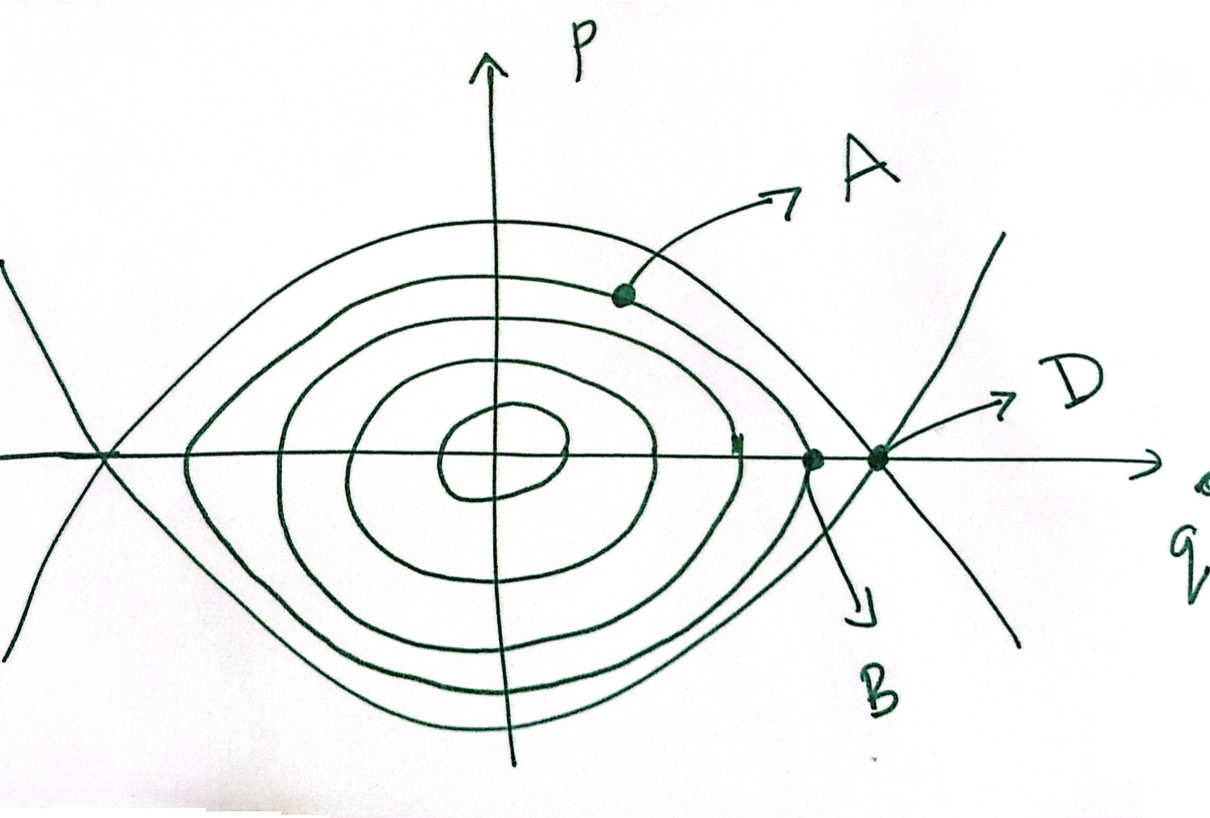
\includegraphics[width=0.5\linewidth]{w.png}
  \caption{Phase portrait}
  \label{fig:boat1}
\end{figure}


\textbf{Background:}
 If we are not on a separatrix, 
then we have the following set of 
coordinates to work with:
$(\vec{p}, \vec{q}) \leftrightarrow (\vec{J}, \vec{\theta}) 
\leftrightarrow (\vec{C}, \vec{\theta})$. The first set are
the standard canonical variables, the second is action-angle variables,
and $\vec{C}$ is the set of  constants of motion.
$\vec{\theta}$ are angle variables which are canonical to $\vec{J}$,
but not to $\vec{C}$.
Let's define a critical point (CP) as one 
where the $dC_i$'s cease to be linearly independent (LI). 






Refer to the figure (drawn for a 1 DOF system for simplicity).
 Let us move to a point $B$ which is
very close to the CP $D$. Also shown here is the torus 
which contains $B$. $A$ is some point on this torus which can
be reached from $B$ by flowing under the Hamiltonian by some
finite amount.






We have the following set of variables to do
multivariable  calculus with: (i) $(\vec{p}, \vec{q})_A$
(ii) $(\vec{p}, \vec{q})_B$
(iii) $(\vec{J}, \vec{\theta})_A$
(iv) $(\vec{J}, \vec{\theta})_B$
(v) $(\vec{C}_B, \vec{\theta}_A)$.
Here the subscripts denote at what point the
coordinates are to be evaluated.
The above five sets of variables are
clearly connected by some functional transformations.
In fact, the first four set of variables are connected via 
canonical transformations because
(i) $(\vec{p}, \vec{q})  \leftrightarrow (\vec{J}, \vec{\theta}) $ 
is canonical transformation
(ii) Flowing under the Hamiltonian leads to
$(\vec{p}, \vec{q})_A  \rightarrow (\vec{p}, \vec{q})_B $
and induces a canonical transformation.






At a CP, 
$dC_i$ are not LI, and this implies that
(see \href{https://math.stackexchange.com/questions/3603283/differential-1-forms-and-linear-independence}{this} 
and 
\href{https://math.stackexchange.com/questions/95167/covectors-omega1-omegak-are-linearly-dependent-iff-their-wedge-produ}{this} link)
\begin{align}
dC_1 \wedge dC_2 \wedge dC_3 \wedge... = 0   .     \label{1}
\end{align}
So at a point $B$, which is close to the CP $D$,
 the ratio of the  differential volume of the parallelepiped
 in the $\vec{C}_B$ space
to a corresponding differential volume 
of a parallelepiped in the $(\vec{p}, \vec{q})_B$ space approaches 0 
(see Eq. 2.91 of Sean Carroll's book).
This ratio approaches 0 even if the denominator is replaced by
 a differential volume 
of a parallelepiped in the $(\vec{p}, \vec{q})_A$ since points
$A$ and $B$ are connected by canonical transformations and
canonical transformations preserve volumes.
What about the ratio of volumes of 
the differential parallelepiped in the 
$(\vec{C}_B, \vec{\theta}_A)$ space vs that in the
$(\vec{p}, \vec{q})_A$ space?
Let us answer this question after making a choice;
we will justify later that we can always make such a choice.




\textbf{Choice:}
Point A has been chosen so that
the differential volume
$(d \theta_1 \wedge d\theta_2 \wedge...)_A$ at this point does not
blow up.



Now due to Eq.~\ref{1}, and the above choice, the
ratio of the volume 
$(dC_1 \wedge dC_2 \wedge...)_B \wedge
(d \theta_1 \wedge d\theta_2 \wedge...)_A$
of  the differential parallelepiped in the 
$(\vec{C}_B, \vec{\theta}_A)$ space 
to the corresponding volume 
of a parallelepiped in the $(\vec{p}, \vec{q})_A$ space approaches 0.
This leads to
  \begin{align}   
  \left\vert   \frac{\partial (\vec{C}_B, \vec{\theta}_A)}{\partial (\vec{p}, \vec{q})_A} \right\vert & \rightarrow 0,  \\
   \left\vert     \frac{\partial (\vec{C}_B, \vec{\theta}_A)}{\partial (\vec{J}, \vec{\theta})_A}
\frac{{\partial (\vec{J}, \vec{\theta})_A}}{\partial (\vec{p}, \vec{q})_A}  \right\vert  & \rightarrow 0,
~~~~~~\mathrm{chain~rule} \\
 \left\vert    \frac{\partial (\vec{C}_B, \vec{\theta}_A)}{\partial (\vec{J}, \vec{\theta})_A}   \right\vert   &\rightarrow 0, 
 ~~~~~~\mathrm{Jacobian~is~1~for~canonical~transformations}  \\
\left\vert    \frac{\partial (\vec{C}_B, \vec{\theta}_A)}{\partial (\vec{J}_B, \vec{\theta}_A)}   \right\vert &\rightarrow 0, 
  ~~~~~~\text{actions~don't~change~from~one~moves~from}~A~\mathrm{to~}B \\
 \left\vert   \frac{\partial \vec{C}_B}{\partial \vec{J}_B} \right\vert 
   \left\vert    \frac{\partial \vec{\theta}_A}{\partial  \vec{\theta}_A}     \right\vert  &\rightarrow 0, 
   ~~~~~~\mathrm{Jacobian~for~a~block~diagonal~matrix~is~the~product~of~Jacobians~
   for~the~blocks}   \\ 
 \left\vert   \frac{\partial \vec{C}}{\partial \vec{J}}     \right\vert  &    \rightarrow 0.  ~~~~~~\mathrm{Label}~B~\mathrm{dropped~
 since~it~is~valid~for~the~entire~torus }
  \end{align}
In conclusion, $|\partial \vec{C}/\partial \vec{J}| \rightarrow 0$ for an entire torus
which approaches a CP. This equation basically gives us the separatrix since a separatrix
is the limit of a torus that approaches a CP.





\textbf{Justification of the above choice:} My justification is hand-wavy, and should be made mathematically 
more sound. The differential volume
$(d \theta_1 \wedge d\theta_2 \wedge...)$ in the
$\vec{\theta}$ space can't blow up at all the points on a torus even if the 
torus is approaching the CP $D$, such as the torus passing through
$B$ in the figure. This is so because even for such a torus,
the change in $\theta_i$ is $2 \pi$ (which is finite) 
after going through the torus once.
The point $A$ chosen above is such a point where $(d \theta_1 \wedge d\theta_2 \wedge...)$
does not blow up.




\textbf{Loophole in the proof and how to fix it:} 
The method seems to fail when we take $\vec{C} = \vec{J}$. The remedy is that
we dictate $\vec{C}$ to be such that their differentials never blow up.
So it can't be that $\vec{C} = \vec{J}$. In fact, the 
$\vec{C} = (H, J, J_z, L, S_{eff}.L)$ in our paper fits this criterion.





\section{Better proof/argument}



Imagine being at a determinant-blow-up point. 
There are only 2 possibilities. Constants of motion (COM) 
being (1) independent (2) dependent. If it's the latter then we have 
non-integrability. Now, let's focus on the former.
Former implies the actions being dependent. Hence this are not valid
action-angle (AA) coordinates.


Is it possible to perform AA-AA transformation so that the with the
new AA, the determinant blow up problem does not arise. No. Why?
Imagine if it were possible. Then AA-old to AA-new will have unit
determinant, which is equal to action transform determinant
(infinity) times
angle transform determinant (zero) since this AA-AA transform
will be a semi-block diagonal transform (actions depend only on the actions; 
the same can't be said about the angles leaving the upper-right block
full of zeros).

Since we are working with the assumption of independent COMs, 
there is a torus A passing through it. Imagine another torus B
close to it. Now the angular volume ratio (between the two sets of angles)
approaches infinity on torus B, which is impossible since both sets of 
angles run from 0 to 2 $\pi$ on the torus. Hence it's not possible to
find another set of AA which don't give the determinant blow up.



At the determinant blow up point,
AA coordinates fail, which implies that the former assumption 
(that of independent COMs) can't be true by Theorem 11.6 of Fasano-Marmi.
Hence Assumption (2) is the only viable option in the face of the
determinant blow up situation.



\textbf{Last issue:} Why not take $\vec{C} = \vec{J}$? This does not give any 
determinant blow up. Because we want to take $\vec{C}$ whose differentials don't 
become undefined at any point.



Do mention that the naive argument does not work. The argument says that
since discontinuous topologies implies discontinuous action integrals.



\textbf{Important:} You can also check for both the determinant vanishing
and blowing up for hunting the separatrix.



\section{Other approaches to finding the separatrix}


Why prefer the above $|dC/dJ| \equiv f(\vec{C}) = 0$ over looking for points where
$dC_i$'s not LD (linearly dependent) for the following reasons.
\begin{itemize}
\item Naturally, separatrices are labeled by $\vec{C}$. So, it's 
good to give separatrices by an expression which involves 
the $\vec{C}$ directly. This is also easier to explain to 
other people, where the linear dependence criterion is esoteric.
\item The latter uses singular value decomposition and
computes eigenvalues. Think if this is too intensive computation-wise.
\item LIGO parameter estimation gives us the constants of motion and the 
masses, which can be directly fed into the former method to see
if $f(\vec{C}) >0$ or $<0$ (oscillates or rotates). If we try to use the latter 
method, we may need to run the SVD all over again for a new detection
because SVD routine to detect rank-deficiency is a numerical procedure
and every new detection comes with its own new values for $m_1$ and $m_2$. 
\item If we are at a point $(\vec{x}, \vec{p})$ which is not on
a separatrix, it is simple matter to move towards a separatrix by 
computing the gradient of $f(\vec{C})$ in this space 
and follow (or anti-follow) it, depending on the sign of $f(\vec{C})$.
\end{itemize}






\bibliography{pn}

\end{document}
